\documentclass[letterpaper]{report}

% packages to include additional functionality
\usepackage{makeidx}         % allows index generation
\usepackage{graphicx}        % standard LaTeX graphics tool
                             % when including figure files
\usepackage{multicol}        % used for the two-column index
\usepackage[bottom]{footmisc}% places footnotes at page bottom
\usepackage{wrapfig} % for wrapping images with text
\usepackage{color} % for coloring links
\usepackage{fancyvrb}
\usepackage{listings}
\usepackage{verbatim}
\usepackage{alltt}
\usepackage{hyperref}%for including URL
%Start Margins
\addtolength{\oddsidemargin}{-.875in}
\addtolength{\evensidemargin}{-.875in}
\addtolength{\textwidth}{1.75in}
\addtolength{\topmargin}{-.885in}
\addtolength{\textheight}{1.95in}
%End Margins

\begin{document}

\renewcommand{\thesection}{\arabic{section}}

\author{Mallika Kogatam}
\title{CS 595: Assignment 2}

\date{Fall 2014}

% note that this special command is part of the document class
% and, in addition to creating the title page, also inserts the 
% current date on the page
\maketitle

\tableofcontents
\newpage

% include other tex files so we don't have one huge document to scroll through

 


\section{Problem 1}
\label{part1}
\begin{enumerate}
\item Write a Python program that extracts 1000 unique links from
Twitter.  You might want to take a look at:

http://thomassileo.com/blog/2013/01/25/using-twitter-rest-api-v1-dot-1-with-python/

\item But there are many other similar resources available on the web.  Note
that only Twitter API 1.1 is currently available; version 1 code will
no longer work.

\item Also note that you need to verify that the final target URI (i.e., the
one that responds with a 200) is unique.  You could have different
shortened URIs for www.cnn.com.  For example, 

http://cnn.it/1cTNZ3V\\
http://t.co/BiYdsGotTd

\item Both ultimately redirect to cnn.com, so they count as only 1 unique URI.
Also note the second URI redirects twice -- don't stop at the first
redirect.

You might want to use the search feature to find URIs, or you can
pull them from the feed of someone famous (e.g., Tim O'Reilly).

Hold on to this collection -- we'll use it later throughout the semester.
\end{enumerate}

\subsection{Solution}

Extracting 1000 unique links from Twitter was more complex endeavor than expected. 

The following steps were taken in order to get the links 
\begin{enumerate}
\item First the key and secret keys for OATH and API are collected by registering an Application in Twitter with an account.
\item TwitterSearch package is used to get the URI's from tweets for a specific keyword.
\item All the URI's that are present in the tweets got from the search for a particular key word are put in an array set. By keeping it in a set eliminates the redundant entries. 
\item Then checked whether the Url's are redirected to same website or not and also checked whether the extracted url is working or not. 
\item To get the URLs form tweets it take so long and apart from that i faced the 429 error which says "too many requests", so i will have to waiti for 15 minutes to run the next time. 
\item When I searched for 5000 urls form the tweets I got only 480 unique links out of them. so I kept incrasing the count to get 1000 unique links
\item When I increased the count to 17000 I got 1500 unique links and this script took almost 40 minutes to run. 
\item I could not even split the program into two different script as there might be repetition in the output got from both the scripts so I will have to run it in a single script.    
\item This way collected 1000 URI's for keyword "twitter". 
\end{enumerate}
\newpage
\subsection{Code Listing}
Here is the python code that is used to collect Thousand URL's from twitter. 


\lstinputlisting[language=Python,breaklines = true,frame=single,caption={Python program for acquiring 1000 unique links for a given keyword}, label=lst:q1-1,captionpos=b,numbers=left,showspaces=false,showstringspaces=false,basicstyle=\footnotesize]{list_unique_links.py}
\newpage
\subsection{Results}


\verbatiminput{samplelinks.txt}




\section{Problem 2}
\label{part2}
\begin{verbatim}

Download the TimeMaps for each of the target URIs.  We'll use the mementoweb.org 
Aggregator, so for example:

URI-R = http://www.cs.odu.edu/

URI-T = http://mementoweb.org/timemap/link/http://www.cs.odu.edu/

You could use the cs.odu.edu aggregator:

URI-T = http://mementoproxy.cs.odu.edu/aggr/timemap/link/1/http://www.cs.odu.edu/

But be sure to say which aggregator you use -- they are likely to give
different answers.

Create a histogram of URIs vs. number of Mementos (as computed from
the TimeMaps).  For example, 100 URIs with 0 Mementos, 300 URIs
with 1 Memento, 400 URIs with 2 Mementos, etc.

See: http://en.wikipedia.org/wiki/Histogram

Note that the TimeMaps can span multiple pages.  Look for links like:

<http://mementoweb.org/timemap/link/1000/http://www.cnn.com/>;rel="timemap"; 
type="application/link-format"; from ="Sun, 08 Jul 2001 21:30:54 GMT"

This indicates another page of the TimeMap is available.  There can be 
many pages to a TimeMap.
\end{verbatim}

\subsection{Solution}
\begin{enumerate}
\item In order to compute the mementos for a link we need the TimeMap for each link from the file containing many links which is an out from the first question.
\item I used "http://mementoweb.org/timemap/link/" because it worked better than http://mementoproxy.cs.odu.edu/aggr/timemap/link/1.And the mementoproxy provided cs department was very slow.   
\item After finding the Time Map for each link parse them and count the mementos.
\item When the request that generate a 404 are recorded as having 0 mementos.and these mementos are counted using a regular expression.
\item I have written Two functions named getTimeMap\(url\) which get the timemaps for each link provided and countMementos\(mem\_url\) which counts the mementos for each timemap generated by the other function. 
\item There can be many pages to a TimeMap.so written a while loop which checks for any timemaps which directs to an other page and found the total count of mementos

\item Finally extracting the mementos and the url name.  
  
\end{enumerate}
\newpage
\subsection{Code Listing}
\subsubsection{mementocount.py}
\lstinputlisting[language=Python,breaklines = true,frame=single,caption={Python program for counting mementos}, label=lst:q1-1,captionpos=b,numbers=left,showspaces=false,showstringspaces=false,basicstyle=\footnotesize]{mementocount.py}
\newpage
\subsubsection{histogram.R}
\lstinputlisting[language=R,breaklines = true,frame=single,caption={R program for generating the histograms for Question 2}, label=lst:q2R,captionpos=b,numbers=left,showspaces=false,showstringspaces=false,basicstyle=\footnotesize]{histogram.R}
\begin{enumerate}
\item Initial I created a histogram with the output i got from the countmementos.py but the graph looked like in the Figure 1 in page 15
\item There is  
\item There are 500 links with 0 mementos and 90 links with more than 1000 mementos and 59 links with 1 memento and 30 links with 2 and other links have mementos mostly under 500. which means majority of the links fall under 1000 mementos. 
\item When plotted the histogram for the above data we get Figure 1 which does not give any proper visualization 
\item I am not satisfied with the figure 1, so i made few changes in order get a decent histogram.
\item So i stripped out the mementos which are grater than 1000 as there are only 90 so this data gives Figure 2 in page 10 which seems little better than the previous one
\item  If we focus more on the highest number of records,mementos less than 200 then the plot actually begins to look more like a histogram in Figure in page 11 
\end{enumerate}

\newpage
\subsection{Results}
\subsubsection{Output for the mementocount.py}
\verbatiminput{samplemementos.txt}
\newpage
\subsubsection{Histograms}
\begin{figure}[ht]    
    \begin{center}
        
\includegraphics[scale=0.60]{q2-histogram1.png}
        \caption{Histogram 1}
        \label{Histogram 1}
    \end{center}
\end{figure}
\newpage
\begin{figure}[ht]    
    \begin{center}
        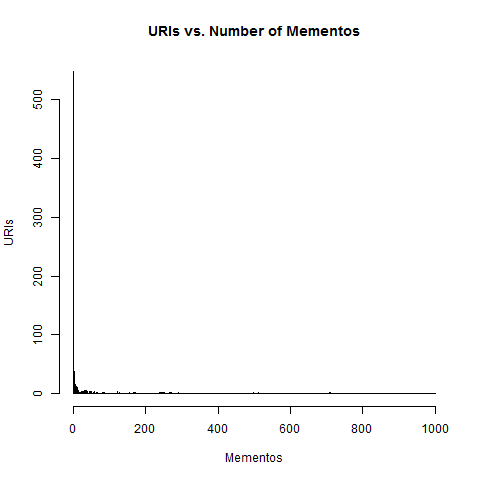
\includegraphics[scale=0.60]{q2-histogram2.png}
        \caption{Histogram 2}
        \label{Histogram 2}
    \end{center}
\end{figure}
\newpage
\begin{figure}[ht]    
    \begin{center}
        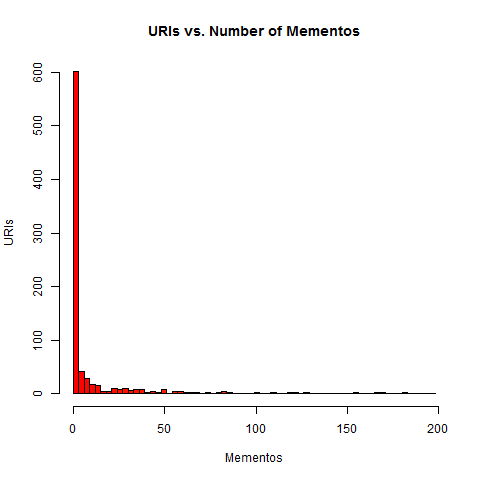
\includegraphics[scale=0.60]{q2-histogram3.png}
        \caption{Histogram 3}
        \label{Histogram 3}
    \end{center}
\end{figure}
\newpage
\section{Problem 3}
\label{part3}
\begin{verbatim}
Estimate the age of each of the 1000 URIs using the "Carbon Date" tool:

http://ws-dl.blogspot.com/2013/04/2013-04-19-carbon-dating-web.html

Note: you'll have better luck downloading and installing the tool 
rather than using the web service (which will run slowly and likely
be unreliable).

For URIs that have > 0 Mementos and an estimated creation date,
create a graph with age (in days) on one axis and number of mementos
on the other.

\end{verbatim}
\subsection{Solution}
\begin{enumerate}

\item Downloaded the carbon tool provided and installed as instructed in the readme file. 
\item From some test runs, it became apparent that the Carbon Date tool takes between 1 and 7 minutes to query all of its services for a given URI. 
\item So getting the dates for all the 1000 URI's from a single script will take more than 36 hours so i executed 5 scripts in 5 different Linux servers which let me extract all the links in 12 hours. 
\item Made changes to local.py from the carbon tool 
in order to read 1000 URI's from a text file and write back the result(time,URI) into an other text file
\item Getting the dates was not enough, because we need the age of each link. 
\item I have written a small python program(caldays.py) which will take the date got from the Carbon Date tool and calculated the days 
\item We will have to create a graph for the links which have >0 mementos and the days for that link
\item So inorder to filter the links which have mementos>0 and get the days, i have written an other simple python program  memvsdays.py.
\item memvsdays.py will collect the data which we need to build a graph for URIs that have > 0 Mementos and the days . 

\end{enumerate}
\newpage
\subsection{Code Listing}

\subsubsection{local.py}
\lstinputlisting[language=Python,breaklines = true,frame=single,caption={Python program for getting creation date for URI's}, label=lst:q1-1,captionpos=b,numbers=left,showspaces=false,showstringspaces=false,basicstyle=\footnotesize]{local1.py}
\newpage
\subsubsection{cladays.py}
\lstinputlisting[language=Python,breaklines = true,frame=single,caption={Python program for calculating the age of URI's}, label=lst:q1-1,captionpos=b,numbers=left,showspaces=false,showstringspaces=false,basicstyle=\footnotesize]{caldays.py}
\newpage
\subsubsection{memvsdays.py}
\lstinputlisting[language=Python,breaklines = true,frame=single,caption={Python program for collecting Mementos versus days}, label=lst:q1-1,captionpos=b,numbers=left,showspaces=false,showstringspaces=false,basicstyle=\footnotesize]{memvsdays.py}
\subsubsection{q3graph.R}
\lstinputlisting[language=R,breaklines = true,frame=single,caption={R program for generating the histograms for Question 2}, label=lst:q2R,captionpos=b,numbers=left,showspaces=false,showstringspaces=false,basicstyle=\footnotesize]{q3graph.R}
\newpage
\subsection{Results}
\subsubsection{carbondates.txt}

\verbatiminput{samplelinks.txt}

\newpage
\subsubsection{carbonday.txt}

\verbatiminput{carbondates.txt}
\newpage
\subsubsection{memvsday.txt}
\verbatiminput{memvsday.txt}
\newpage
\subsubsection{q3-scatterplot}
\begin{figure}[ht]    
    \begin{center}
        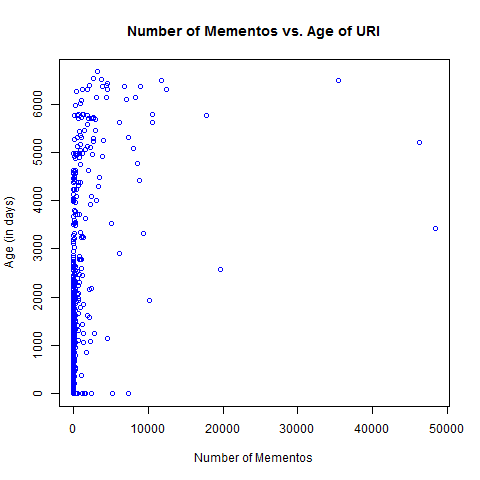
\includegraphics[scale=0.60]{q3-scatterplot.png}
        \caption{ScatterPlot}
        \label{scatterPlot}
    \end{center}
\end{figure}

\bibliographystyle{plain}
\bibliography{a2}
\nocite{*}

\end{document}

